\documentclass[a4paper, 12pt]{report}
\usepackage{geometry}
\geometry{a4paper,hmargin={3cm,2.5cm},vmargin={2.5cm,2.5cm}}

\usepackage{geometry}
\geometry{
    a4paper,
    headheight=15pt,
    hmargin={3cm,2.5cm},
    vmargin={2.5cm,2.5cm}
}
 
\usepackage{amsfonts} % if you want blackboard bold symbols e.g. for real numbers
\usepackage{multicol}
\usepackage{float}
\usepackage{blindtext}
\usepackage{fancyhdr}
\pagestyle{fancy}
\usepackage{hyperref}
\usepackage{amsmath} % for 'bmatrix' environment
\usepackage{tikz}
\usetikzlibrary{calc}
\usepackage{eso-pic}
\usepackage{lipsum}
\usepackage{longtable}
\setlength{\parindent}{0em}
\setlength{\parskip}{1em}
\usepackage{biblatex} %Imports biblatex package
\addbibresource{main.bib} %Import the bibliography file
\usepackage{scrextend}
\usepackage{subfig}
\usepackage{graphicx} % for jpeg or pdf pictures
\usepackage{lmodern}
\usepackage{minted}
\usepackage{colortbl}

\hypersetup{
    colorlinks=true,
    linkcolor=blue,
    filecolor=magenta,      
    urlcolor=cyan,
}

%\lhead{}
%\rhead{Project Report - Preferential Attachment with machine learning}
%\lfoot{Open University of Israel - Dept. of Mathematics and Computer Science}

\begin{document}

%========================== begin of title page ================================ %
% The frontmatter environment for everything that comes with roman numbering
\newenvironment{frontmatter}{}{}
\begin{frontmatter}
%%%%%%%%%%%%%%%%%%%%%%%%%%%%%%%%%%%%%%%%%%%%%%%%%%%%%%%%%%%%%%%%%%%
\begin{titlepage}
%\AddToShipoutPictureBG
\begin{center}
\textup{\large \textbf{The Open University of Israel}}\\[0.5cm]
\textbf{\large Department of Mathematics and Computer Science}

%-------------------------------------- Figure -----------------------------------

\begin{center}
\begin{figure}[h]  %h means here other options t , b, p, etc.
\centering

\includegraphics[width=0.3\linewidth]{./logo}
\end{figure}
\end{center}

%---------------------------------------------------------------------------------

\textup{\large A PROJECT REPORT\\[0.4cm]ON}\\[0.4cm]
\begin{LARGE}
{\textbf {Preferential Attachment }}\\
{\textbf {using machine learning }}\\[1cm]
\end{LARGE}
\textit{SUBMITTED BY}\\[0.3cm]
\begin{large}
\textbf{YOSSI COHEN}\\[0.3cm]
\end{large}
\textit{THE OPEN UNIVERSITY}\\[1cm]
\textit{UNDER THE GUIDANCE OF}\\[0.3cm]
\begin{large}\textbf{PROF. YOSSI GIL}\\[0.3cm]\end{large}
\textit{THE TECHNION}\\[1cm]
\textit{(2020-2021)}
\vfill
\end{center}
\end{titlepage}

%========================== end of title page ================================ %

%------------------------------ ACKNOWLEDGEMENT --------------------------------
\begin{center}
{\Large{\bf{\textit{ACKNOWLEDGEMENT}}\\[2cm]}}
\end{center}

\par\textit{I would like to thank {\bf Prof. Yossi Gil} for encouraging me to go ahead and for his continuous guidance with the project and assistance in preparing this report.}

\par\textit{I would also like to thank all those, who have directly or indirectly helped me for the completion of the work during this project.}

%========================= table of contents ================================= %
\tableofcontents
\listoffigures
\listoftables

%%%%%%%%%%%%%%%%%%%%%%%%%%%%%%%%%%% Abstract %%%%%%%%%%%%%%%%%%%%%%%%%%%%%%%%%%%%
%\newpage
\begin{abstract}
Many of the things that we measure have a \textit{typical value} around which individual measurements are centred. A simple example would be the heights of human beings. Most adult human beings (in the U.S) are about 180 cm tall. There is some variation around this figure, notably depending on sex, but we never see people who are 10 cm tall, or 500 cm. Other examples would be e.g., shoe sizes and speed of cars on the motorway.

However, not all things we measure are peaked around a typical value. Some vary over an enormous dynamic range, sometimes many orders of magnitude. 

When the probability of measuring a particular value of some quantity varies inversely as
a power of that value, the quantity is said to follow a \textit{power law}, also known as \textit{Zipf’s law} or the \textit{Pareto distribution}. 

Power laws appear widely in physics, biology, earth and planetary sciences, economics and finance, computer science, demography and social sciences. For instance, the distributions of the sizes of cities, earthquakes, forest fires, solar flares, moon craters and people’s personal fortunes all appear to follow power laws.

The origin of power-law behaviour has been a topic of debate in the scientific
community for more than a century.

In his paper "Power laws, Pareto distributions and Zipf’s law", Newman review some of the empirical evidence for the existence of power-law forms and the theories proposed to explain them.


{\bf In this project} we show, contrary to the common claim, that a key property of such \textit{power law} distribution, concretely  \textit{Yule-Simon distribution}, can be estimated with a reasonable accuracy using machine learning methods.

\vspace{0.3cm}

\textbf{Keywords - }\it{\textbf{Preferential Attachment, Machine Learning.}}
\end{abstract}
%================================================ %
% The frontmatter environment for everything that comes with roman numbering %
\end{frontmatter}
%%%%%%%%%%%%%%%%%%%%%%%%%%%%%%%%%%%%%%%%%%%%%%%%%%%%%%%%%%%%%%%%%%%%%%%%%%%%%%%%%%%%%%%%%%%%%%%%

\newpage
\pagenumbering{arabic}
%%%%%%%%%%%%%%%%%%%%%%%%%%%%%%%%%%%% MAIN TEXT STARTS HERE %%%%%%%%%%%%%%%%%%%%%%%%%%%%%%%%%%%%%
\chapter{INTRODUCTION}

\section{Background}
TODO

Here I intend to introduce some examples of power law distributions and the mathematical background to explain them (repeat key topics from Newman`s paper)

\section{Previous work}
TODO

Describe key points from Newman's paper

\section{Motivation}
TODO

Here I intend to quote Newman's claim that alpha cannot be estimated correctly using line fit methods on the histogram logarithmic binning (page 5).

I want to emphasize that if machine learning methods can estimate alpha correctly (with an acceptable error) than this preliminary result motivates further investigation on harnessing such methods for identifying power law distributions and maybe classifying distributions as such.

\pagebreak
\section{Yule process}
\par \textit{Preferential Attachment} may be realized using the \textit{Yule process}  \cite{yule-simon-distribution}.

\par An example \textit{Yule process} is implemented by following procedure:
\par Distribute $N >> 1$ balls among urns iteratively using \textit{preferential attachment} policy.

At each step, add a urn with initial $k_0$ balls and distribute $m$ balls among urns with probability proportional to the number of balls in each urn.\\
Run as many iterations as necessary to distribute all $N$ balls.

\par Parameters:
\begin{addmargin}[1cm]{1cm}% 1cm left, 1cm right
    $N: N >> 1$, the total number of balls we wish to distribute.\\
    $m: 1 <= m <= 10$, the number of balls distributed at each iteration.\\
    $k_0: 1 <= k_0 <= 10$, the initial number of balls for a newly created urn.
\end{addmargin}

{\fontfamily{qcr}\selectfont
As an example: N = 10000; k0 = 10; m = 3
}

\begin{figure}[ht]
\centering
    % Requires \usepackage{graphicx}
    \subfloat[]{
        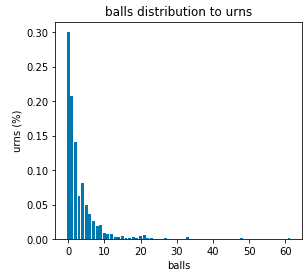
\includegraphics[width=0.25\textwidth]{yule-histogram}
        \label{fig:1a}
    }
    \hspace{0.5cm}
    \subfloat[]{
        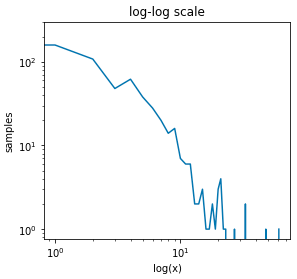
\includegraphics[width=.25\textwidth]{yule-log}
        \label{fig:1b}
    }
    \hspace{0.5cm}
    \subfloat[]{
        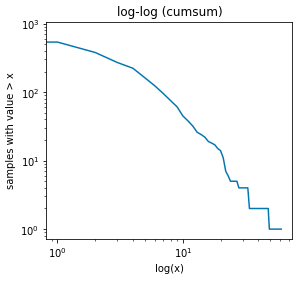
\includegraphics[width=.25\textwidth]{yule-log-cumsum}
        \label{fig:1c}
    }
    \label{fig:1}
    \caption[Yule process histograms]{
        $(a)$ A histogram of $N=10,000$ balls distributed to urns with \textit{Yule distribution}.
        $(b)$ The same histogram on logarithmic scale.
        $(c)$ A cumulative histogram of the same data.
    }
\end{figure}

\pagebreak
\chapter{PROBLEM  STATEMENT}

\section{Problem Statement}
\par The first line of the first paragraph under each heading should start from left-hand margins without indentation.  Text of abstract should be typed in Times New Roman, 12pt. Keywords should be written in Times New Roman, 12pt, Italic.

\section{Explanation}
\par The first line of the first paragraph under each heading should start from left-hand margins without indentation.  Text of abstract should be typed in Times New Roman, 12pt. Keywords should be written in Times New Roman, 12pt, Italic.\\
\begin{table}[h]

\begin{center}
 \begin{tabular}{||c|c|c|c||} 

 \hline
 Col1 & Col2 & Col2 & Col3 \\ [0.5ex] 
 \hline\hline
 1 & 6 & 87837 & 787 \\ 
 \hline
 2 & 7 & 78 & 5415 \\
 \hline
 3 & 545 & 778 & 7507 \\
 \hline
 4 & 545 & 18744 & 7560 \\
 \hline
 5 & 88 & 788 & 6344 \\ 
 \hline
\end{tabular}
\caption{table name}
\end{center}
\end{table}

\chapter{SOFTWARE REQUIREMENT SPECIFICATION}

\section{Software and Hardware Requirement}
\par The first line of the first paragraph under each heading should start from left-hand margins without indentation.  Text of abstract should be typed in Times New Roman, 12pt. Keywords should be written in Times New Roman, 12pt, Italic.

\subsection{Description}
\par The first line of the first paragraph under each heading should start from left-hand margins without indentation.  Text of abstract should be typed in Times New Roman, 12pt. Keywords should be written in Times New Roman, 12pt, Italic.

\chapter{PROJECT IMPLEMENTATION}

\section{Dataset}
\label{dataset}

\par The datasets used in the project were generated using the \textbf{\textit{yulesimon}} distribution from \textbf{\textit{scipy.stat}} package.

\par As an example, the following will generate $1000$ random numbers for a given $alpha=\alpha$
\begin{equation}
\label{eq:1}
r = yulesimon.rvs(alpha=\alpha, size=1000)
\end{equation}
The $generate\_data()$ function uses \ref{eq:1} to draw $N$ random samples for each $\alpha$ in the range: $[min\_alpha, max\_alpha]$ with $S$ $yulesimon.rvs$ calls for each $\alpha$, yielding the following dataset:\\
(Concatenated as a single matrix $YS = [(M * S), N]$)
\begin{itemize}
  \item $N$ (columns): number of samples drawn for a given $\alpha$
  \item $M$: number of different $\alpha$ generated in the range: [$min\_\alpha$, $max\_\alpha$]
  \item $S$: number of samples per $\alpha$ (number of calls to $yulesimon.rvs$ with same $\alpha$)
\end{itemize}

\[
samples(\alpha_1) = \begin{bmatrix} 
    r^{(\alpha_1)}_{1,1} & r^{(\alpha_1)}_{1,2} & \dots & r^{(\alpha_1)}_{1,N} & \\
    r^{(\alpha_1)}_{2,1} & r^{(\alpha_1)}_{2,2} & \dots & r^{(\alpha_1)}_{2,N} & \\
    \vdots & \ddots & \vdots & \\
    r^{(\alpha_1)}_{S,1} & r^{(\alpha_1)}_{S,2} & \dots & r^{(\alpha_1)}_{S,N} & \\
\end{bmatrix}
\]

\[
samples(\alpha_2) = \begin{bmatrix} 
    r^{(\alpha_2)}_{1,1} & r^{(\alpha_2)}_{1,2} & \dots & r^{(\alpha_2)}_{1,N} & \\
    r^{(\alpha_2)}_{2,1} & r^{(\alpha_2)}_{2,2} & \dots & r^{(\alpha_2)}_{2,N} & \\
    \vdots & \ddots & \vdots & \\
    r^{(\alpha_2)}_{S,1} & r^{(\alpha_2)}_{S,2} & \dots & r^{(\alpha_2)}_{S,N} & \\
\end{bmatrix}
\]

\[
...
\]

\[
samples(\alpha_M) = \begin{bmatrix} 
    r^{(\alpha_M)}_{1,1} & r^{(\alpha_M)}_{1,2} & \dots & r^{(\alpha_M)}_{1,N} & \\
    r^{(\alpha_M)}_{2,1} & r^{(\alpha_M)}_{2,2} & \dots & r^{(\alpha_M)}_{2,N} & \\
    \vdots & \ddots & \vdots & \\
    r^{(\alpha_M)}_{S,1} & r^{(\alpha_M)}_{S,2} & \dots & r^{(\alpha_M)}_{S,N} & \\
\end{bmatrix}
\]

\par A histogram $H$ is then created for rows of $[YS]$ where: 
\begin{equation}
\label{eq:2}
\textbf {nbins} = max(YS)
\end{equation}

\[
{\textbf H} = \begin{bmatrix} 
    histogram(samples(\alpha_1), nbins) & \\
    histogram(samples(\alpha_2), nbins) & \\
    \vdots & \\
    histogram(samples(\alpha_S), nbins) & \\
\end{bmatrix}
\]

\par Finally, we apply $log_{10}$ on $H$ rows:
\begin{equation}
\label{eq:3}
    {\textbf X} = log_{10}(H)
\end{equation}

We set:
\begin{equation}
\label{eq:4}
{\textbf y} = \begin{bmatrix} 
    \alpha_1 & \\
    \alpha_2 & \\
    \vdots & \\
    \alpha_M & \\
\end{bmatrix}
\end{equation}

\begin{itemize}
  \item note: $y$ contains $S$ copies for each of $\alpha_1...\alpha_M$ for total length of $[S*M]$
\end{itemize}

\par The $generate\_data()$ function returns: $(X, y, nbins)$ as an input for the learning process.

\pagebreak
\par An example of a single row in $X = log(H)$ is shown in figure  \ref{fig:2}

\begin{figure}[h]
\centering
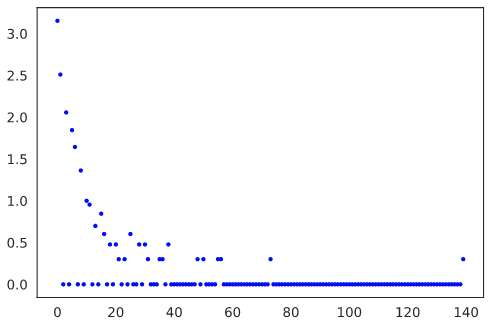
\includegraphics[width=0.7\linewidth]{./dataset}
\caption[Yule-Simon log-scale]{$X = log(H)$ for $\alpha\in[2.0,3.0], N=2048$ \\(140 bins = $max(X)$)}
\label{fig:2}
\end{figure}

\textit{Note}: We will see later that padding bins with zero value at the right end improves the $NN$ model accuracy (figure  \ref{fig:3})

\begin{figure}[h]
\centering
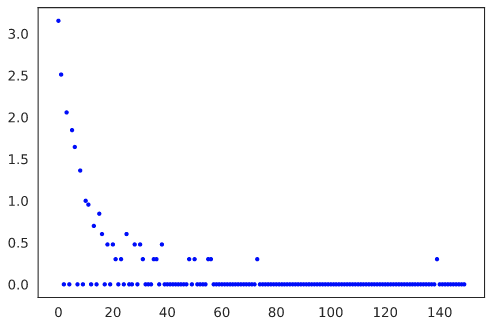
\includegraphics[width=0.7\linewidth]{./dataset-zeros}
\caption[Yule-Simon log-scale with zero padding]{Yule-Simon samples for $\alpha\in[2.0,3.0], N=2048$ \\(right padding zero bins)}
\label{fig:3}
\end{figure}

\pagebreak
\section{DNN}
\par As stated in \cite{newman}, In practical situations we would often like to estimate $\alpha$ from observed data. One way to do this would be to fit the slope of the line in plots like figures (\ref{fig:1b}), (\ref{fig:1c}) Unfortunately, it is known to introduce systematic biases into the value of the exponent $\alpha$, so it should not be relied
upon.

\par \textit{DNN (Deep Neural Network)}, not like simple line-fit models, can learn complex patterns. Thus, the first approach used in this project was a \textit{Regression DNN}.

\subsection{DNN Model training}
The \textit{DNN} model was implemented using \textit{Keras} under \textit{Jupyter Notebook}.

\par The neural network has an input layer which is fed with the dataset described in section \ref{dataset}. It has couple of fully connected hidden layers with \textit{relu} activation and an output layer with a \textit{linear} activation. All layers use batch normalization, \textit{Adam} optimizer, kernel and activation \textit{regularization}. The loss function used is \textit{MSE}.

\par We have made little attempts to optimize the parameters of the network, and
so improved performance may be obtained by exploring other values.

\par Input to the network has been splitted to \textit{TRAIN}, \textit{VALIDATION} and \textit{TEST} sets.

\par Model training used \textit{early stopping} and \textit{reduce learning-rate on plateau}.\\
Training used \textit{batch size} of $32$ and couple of hundred \textit{epochs}.

\textit{Learning Curves} (train/validation) have been used to identify and eliminate \textit{overfitting}.

\pagebreak
\subsection{Experiments}
In order to streamline experiments, a $trial()$ helper function has been defined.\\
$trial()$ runs several iterations as defined by the following arguments:

\begin{itemize}
  \item $N\_range$: a set $\{I\}$ where $\{N = 2^{i\in I}\}$ are the number of samples to draw from \textit{yulesimon} distribution for a given $\alpha$.
  \item $hstack\_zeros$: whether to right append zeros to the generated \textit{dataset}.
  \item $\{random\_states\}$: a set of random state values to run the trained model in each iteration.
\end{itemize}

$trial()$ uses $generate\_data(N, num\_alphas, samples\_per\_alpha)$ to produce growing size datasets. For each \textit{dataset} generated, $trial()$ creates a corresponding \textit{DNN} model. It then iterates over the given $\{random\_states\}$ set to train and test the model.

\par $trial()$ returns:
\begin{itemize}
  \item $[N]$: the list of $N's$ used in each iteration.
  \item $[sqrt\_mse]$: the corresponding $sqrt(mse)$ for each iteration.
  \begin{itemize}
    \item $sqrt\_mse = sqrt(mean\_squared\_error(\alpha\_test, \alpha\_pred))$
  \end{itemize}
  \item $[avg\_abs\_errors]$: avg of absolute errors for each iteration.
  \begin{itemize}
    \item $avg\_abs\_errors = avg(abs(\alpha\_test - \alpha\_pred))$
  \end{itemize}
  \item $[std\_abs\_errors]$: STD of absolute error for each iteration.
  \begin{itemize}
    \item $std\_abs\_errors = std(avg\_abs\_errors)$
  \end{itemize}
\end{itemize}

\pagebreak
\subsection{DNN results}
\par Running \textit{DNN} on $100$ alphas with 100 samples per alpha yield the following:

\begin{table}[h!]
    \centering
    \begin{tabular}{||c c c||} 
        \hline
        $N$ & input-shape & $avg(sqrt(mse(\alpha)))$ \\ [0.5ex] 
        \hline\hline
        32 & (10000, 34) & 0.04326 \\ 
        \hline
        64 & (10000, 20) & 0.01430 \\
        \hline
        128 & (10000, 46) & 0.01480 \\
        \hline
        256 & (10000, 21) & 0.01041 \\
        \hline
        512 & (10000, 33) & 0.00908 \\ 
        \hline
        1024 & (10000, 63) & 0.00985 \\ 
        \hline
        2048 & (10000, 140) & 0.01002 \\ 
        \hline
    \end{tabular}
    \caption[$mse(\alpha)$ for $DNN$]{$DNN - avg(sqrt(mse(\alpha)))$}
    \label{table:1}
\end{table}

\textit{note}: for each $N$, we run several train/test cycles, each with different random-state and average the results:
\begin{minted}{python}
for rs in random_states:
    model = train(model, X_train, y_train, ..., random_state=rs)
    y_pred = model.predict(X_test)
    sqrt_mse = sqrt(mse(y_test, y_pred))
    avg_sqrt_mse += sqrt_mse
    ...
avg_sqrt_mse \= len(random_states)
\end{minted}

\subsection{DNN results with zero padding}
\par Running \textit{DNN} on the same input as above with right padding zeros yield the following:
\begin{table}[h!]
    \centering
    \begin{tabular}{||c c c||} 
        \hline
        $N$ & input-shape & $avg(sqrt(mse(\alpha)))$ \\ [0.5ex] 
        \hline\hline
        32 & (10000, 44) & 0.04341 \\ 
        \hline
        64 & (10000, 30) & 0.01435 \\
        \hline
        128 & (10000, 56) & 0.01506 \\
        \hline
        256 & (10000, 31) & 0.01066 \\
        \hline
        512 & (10000, 43) & 0.00798 \\ 
        \hline
        1024 & (10000, 73) & 0.01143 \\ 
        \hline
        2048 & (10000, 150) & 0.00789 \\ 
        \hline
    \end{tabular}
    \caption{$mse(\alpha)$ for $DNN$ with zero padding}
    \label{table:2}
\end{table}

\pagebreak
\subsection{DNN additional experiments}
Before moving to describe the $CNN$ based model, it should be mentioned that several additional experiments were taken based on the $DNN$ model. Two of them are described here.

Trying to help the $DNN$ model to capture the shape of the input, a \textit{sliding-avg} and a \textit{sliding-sum} manipulations on the input have been taken.

\subsubsection{DNN sliding-avg}
By an example, suppose a row of the input is:
\begin{minted}{python}
    [1 2 3 4 5 6 7]
\end{minted}

The \textit{sliding-avg} works row-wise on window sizes of $2^i$ where $i \in \{1,2,...\}$.

In the example above, valid window sizes are:
\begin{minted}{python}
    window_sizes: [2, 4]
\end{minted}

The \textit{sliding-avg} copy a row of the input as is ($1..7$). Then, starts by sliding a window of size 2 (stride=1) and appends the avg. of every two elements ($avg(1,2)$, $avg(2,3)$, ...). Then it begins from the start with a sliding a window of size 4 (stride=1) averaging every 4 elements. The output follows:
\begin{minted}{python}
    [1.  2.  3.  4.  5.  6.  7.  1.5 2.5 3.5 4.5 5.5 6.5 2.5 3.5 4.5 5.5]
\end{minted}

\subsubsection{DNN sliding-sum}
The \textit{sliding-sum} goes the same way as the \textit{sliding-avg} but appends the sum-elements of $window\_size=2$, then $window\_size=4$, etc. The output follows:
\begin{minted}{python}
    [1.  2.  3.  4.  5.  6.  7.  3 5 7 9 11 13 10 14 18 22]
\end{minted}

\subsubsection{Sliding-windows results}
It appeared that the sliding methods didn't improve performance.

\pagebreak
\section{CNN}
Although $DNN$ yields relatively acceptable errors ($\approx 0.01$ for $N>=64$), a $~CNN$ model ($Conv1D$) has been investigated.

A $Conv1D$ layer creates a convolution kernel (filter) that is convolved with its input over a single spatial (or temporal) dimension to produce a tensor of outputs.

Filters learn feature representations of the input. The more representations used the better the performance will be (generally not always, having more filters than needed can also lead to overfitting).

In the first experiment we used a $Conv1D$ with 32-filters of size 3 and a $relu$ activation, followed by max-pooling $(pool\_size=2)$ and two $Dense$ layers $Dense(64, relu)$ and $Dense(1)$. The loss is again $MSE$ and the optimizer used was \textit{Adam}.

The model is fairly simple:
\begin{minted}{python}
def create_cnn_model(n_features, filters=32):
    model = Sequential()
    model.add(Conv1D(32, 3, activation='relu', input_shape=(n_features, 1)))
    model.add(MaxPooling1D(pool_size=2))
    model.add(Flatten())
    model.add(Dense(64, activation='relu'))
    model.add(Dense(1))
    model.compile(loss='mse', optimizer='adam')
    return model
\end{minted}

\subsection{CNN results}
The $CNN$ model was tested the same way as the $DNN$ model using the $trials()$ helper over the same inputs. It yield the following results:

\begin{table}[h!]
    \centering
    \begin{tabular}{||c c c||} 
        \hline
        $N$ & input-shape & $avg(sqrt(mse(\alpha)))$ \\ [0.5ex] 
        \hline\hline
        32 & (10000, 34) & 0.04104 \\ 
        \hline
        64 & (10000, 20) & 0.01080 \\
        \hline
        128 & (10000, 46) & 0.01146 \\
        \hline
        256 & (10000, 21) & 0.00498 \\
        \hline
        512 & (10000, 33) & 0.00365 \\ 
        \hline
        1024 & (10000, 63) & 0.00219 \\ 
        \hline
        2048 & (10000, 140) & 0.00122 \\ 
        \hline
    \end{tabular}
    \caption{$mse(\alpha)$ for $CNN$}
    \label{table:3}
\end{table}

\subsection{CNN results with zero padding}
\par Running \textit{CNN} on the same input as above with right padding zeros yield the following:
\begin{table}[h!]
    \centering
    \begin{tabular}{||c c c||} 
        \hline
        $N$ & input-shape & $avg(sqrt(mse(\alpha)))$ \\ [0.5ex] 
        \hline\hline
        32 & (10000, 44) & 0.04111 \\ 
        \hline
        64 & (10000, 30) & 0.01085 \\
        \hline
        128 & (10000, 56) & 0.01161 \\
        \hline
        256 & (10000, 31) & 0.00483 \\
        \hline
        512 & (10000, 43) & 0.00329 \\ 
        \hline
        1024 & (10000, 73) & 0.00229 \\ 
        \hline
        2048 & (10000, 150) & 0.00110 \\ 
        \hline
    \end{tabular}
    \caption{$mse(\alpha)$ for $CNN$ with zero padding}
    \label{table:4}
\end{table}

\section{CNN multi-layer}
The second $CNN$ experiment used a multi-layer with multiple $Conv1D$ and pooling:

\begin{minted}{python}
def create_cnn_model_multi_layer(n_features, filters=32):
    model = Sequential()
    # conv layer 1
    model.add(Conv1D(filters,
                     kernel_size=7, strides=1, 
                     activation='relu', 
                     input_shape=(n_features, 1)))
    # conv layer 2
    input_size = ( input_size + 2 * padding - kernel_size ) / strides  + 1
    model.add(Conv1D(filters, kernel_size=5, ...) 
    # pooling layer 1
    model.add(MaxPooling1D(pool_size=2))
    # conv layer 3
    model.add(Conv1D(filters, kernel_size=3, ...) 
    # pooling layer 2
    model.add(MaxPooling1D(pool_size=2))
    # flatten
    model.add(Flatten())
    # dense layer 1
    model.add(Dense(64, activation='relu'))
    # output layer
    model.add(Dense(1))
    model.compile(loss='mse', optimizer='adam', metrics=['mse'])
    return model
\end{minted}

\subsection{CNN multi-layer results}
\par Running \textit{CNN multi-layer} on the same input as above yield the following:
\begin{table}[h!]
    \centering
    \begin{tabular}{||c c c||} 
        \hline
        $N$ & input-shape & $avg(sqrt(mse(\alpha)))$ \\ [0.5ex] 
        \hline\hline
        32 & (10000, 44) & 0.04095 \\ 
        \hline
        64 & (10000, 30) & 0.01097 \\
        \hline
        128 & (10000, 56) & 0.01028 \\
        \hline
        256 & (10000, 31) & 0.00474 \\
        \hline
        512 & (10000, 43) & 0.00302 \\ 
        \hline
        1024 & (10000, 73) & 0.00158 \\ 
        \hline
        2048 & (10000, 150) & 0.00096 \\ 
        \hline
    \end{tabular}
    \caption{$mse(\alpha)$ for $CNN$ multi-layer}
    \label{table:5}
\end{table}

\subsection{CNN multi-layer results with zero padding}
\par Running \textit{CNN multi-layer} with zero padding on the same input as above with right padding zeros yield the following:
\begin{table}[h!]
    \centering
    \begin{tabular}{||c c c||} 
        \hline
        $N$ & input-shape & $avg(sqrt(mse(\alpha)))$ \\ [0.5ex] 
        \hline\hline
        32 & (10000, 44) & 0.04150 \\ 
        \hline
        64 & (10000, 30) & 0.01094 \\
        \hline
        128 & (10000, 56) & 0.01075 \\
        \hline
        256 & (10000, 31) & 0.00438 \\
        \hline
        512 & (10000, 43) & 0.00274 \\ 
        \hline
        1024 & (10000, 73) & 0.00159 \\ 
        \hline
        2048 & (10000, 150) & 0.00068 \\ 
        \hline
    \end{tabular}
    \caption{$mse(\alpha)$ for $CNN$ multi-layer with zero padding}
    \label{table:6}
\end{table}

\pagebreak
\section{Methods comparison}
Table \ref{table:7} summarise $\sqrt{mse(\alpha)}$ for $N=2^i~ i\in\{5...11\}$ for the different methods used.
\begin{table}[!h]
    \sffamily
    \scriptsize
    \caption*{
        $z$: right zero padding\\
        $m$: multi-layer CNN
    }
    \centering
    \begin{tabular}{||c c c c c c c||} 
        \hline
        $N$ & $DNN$ & $DNN_z$ & $CNN$ & $CNN_z$ & $CNN_m$ & $CNN_{m,z}$ \\ [0.5ex] 
        \hline\hline
        32 & 0.043260 & 0.043405 & 0.041040 & 0.041108 & 0.040951 & 0.041504 \\ 
        \hline
        64 & 0.014299 & 0.014351 & 0.010801 & 0.010851 & 0.010968 & 0.010939 \\
        \hline
        128 & 0.014803 & 0.015061 & 0.011461 & 0.011613 & 0.010276 & 0.010751 \\
        \hline
        256 & 0.010409 & 0.010662 & 0.004984 & 0.004832 & 0.004736 & 0.004380 \\
        \hline
        512 & 0.009084 & 0.007984 & 0.003653 & 0.003293 & 0.003019 & 0.002745 \\
        \hline
        1024 & 0.009846 & 0.011425 & 0.002195 & 0.002291 & 0.001577 & 0.001586 \\
        \hline
        2048 & 0.010022 & 0.007886 & 0.001215 & 0.001096 & 0.000956 & 0.000675 \\
        \hline
    \end{tabular}
    \caption{$sqrt(mse(\alpha))$ comparison}
    \label{table:7}
\end{table}

Figure \ref{fig:4} displays a (\textit{logarithmic}) plot of the errors for different $N's$ for each of the methods. The performance of the \textit{CNN} methods over the \textit{DNN} stands out.
\begin{figure}[!h]
\centering
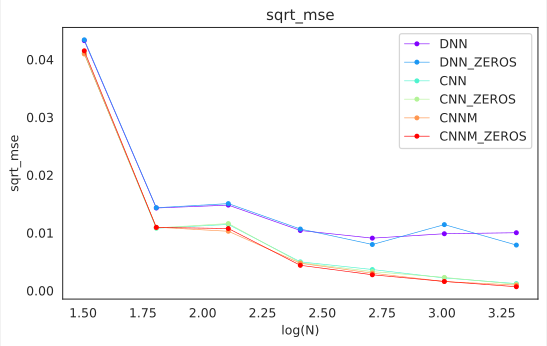
\includegraphics[width=0.7\linewidth]{./sqrt_mse_compare}
\caption{$mse(\alpha)$ comparison}
\label{fig:4}
\end{figure}

Table \ref{table:8} summarise $STD$ of the different methods used.
\begin{table}[!h]
    \sffamily
    \scriptsize
    \centering
    \begin{tabular}{||c c c c c c c||} 
        \hline
        $N$ & $DNN$ & $DNN_z$ & $CNN$ & $CNN_z$ & $CNN_m$ & $CNN_{m,z}$ \\ [0.5ex] 
        \hline\hline
    	32 & 0.023159 & 0.023944 & 0.025286 & 0.025220 & 0.025482 & 0.024870 \\
    	\hline
    	64 & 0.006112 & 0.005835 & 0.007213 & 0.007136 & 0.007140 & 0.007112 \\
    	\hline
    	128 & 0.007661 & 0.007169 & 0.007652 & 0.007497 & 0.006669 & 0.006585 \\
    	\hline
    	256 & 0.003591 & 0.002905 & 0.003501 & 0.003425 & 0.002951 & 0.003059 \\
    	\hline
    	512 & 0.002553 & 0.002169 & 0.002071 & 0.002125 & 0.001828 & 0.001911 \\
    	\hline
    	1024 & 0.001992 & 0.003733 & 0.001593 & 0.001700 & 0.001009 & 0.001019 \\
    	\hline
    	2048 & 0.003038 & 0.001441 & 0.000609 & 0.000606 & 0.000533 & 0.000425 \\
	\hline
    \end{tabular}
    \caption{$STD$ comparison}
    \label{table:8}
\end{table}

\newpage
\subsection{T-TEST}
Is the difference in performance between two machine learning models real, or due to a statistical fluke? Statistical significance tests are designed to address this question.

\textit{T-TEST} compares two averages (means) and tells us if they are different from each other and how significant the differences are; In other words it lets us know if those differences could have happened by chance.

We will use a paired \textit{T-TEST} to compare the results of the different methods used in this project, particularly, the results of \textit{DNN} versus those of \textit{CNN}.

The model\_compare function accepts two models and compares the significance of the difference between their performance (see pseudo code below):

\begin{minted}{python}
from scipy import stats

def model_compare(nn1='DNN', nn2='CNN', N_pow, num_tests)
    N = 2**N_pow
    for i in range(num_tests):
        random_state = random.randint(0,100)
        X, y = generate_data(N, random_state, ...)
        X_train, X_test, y_train, y_test = train_test_split(X, y)
        for nn in [nn1, nn2]:
            model = create_model(nn, X_train, random_state)
            train(model, X_train, y_train, ..., random_state)
            y_pred = model.predict(X_test_model)
            sqrt_mse = np.sqrt( mean_squared_error(y_test, y_pred) )
    a = [ sqrt_mse results of nn1 in each random_state ]
    b = [ sqrt_mse results of nn2 in each random_state ]

    return stats.ttest_rel(a, b)
\end{minted}

Table \ref{table:9} summarize the results of comparing some models.\\
We can see $ttest(DNN, CNN)$ for $N >= 256$ pops out, compatible with Figure \ref{fig:4}.

\begin{table}[h!]
    \scriptsize
    \centering
    \begin{tabular}{||c c c c c||} 
        \hline
        $nn1$ & $nn2$ & $N$ & num\_tests & ttest-$p$ \\ [0.5ex] 
        \hline\hline
        $DNN$ & $DNN_z$ & 64 & 10 & 0.23833 \\ 
        \hline
        $DNN$ & $DNN_z$ & 256 & 5 & \textbf{0.04087} \\ 
        \hline
        $DNN$ & $CNN$ & 64 & 10 & 0.47183 \\ 
        \hline
        $DNN$ & $CNN$ & 128 & 5 & 0.08147 \\ 
        \hline
        \rowcolor{yellow}
        $DNN$ & $CNN$ & 256 & 5 & \textbf{0.01962} \\ 
        \hline
        \rowcolor{yellow}
        $DNN$ & $CNN$ & 1024 & 5 & \textbf{0.00776} \\ 
        \hline
        $CNN$ & $CNN_z$ & 64 & 10 & 0.44374 \\ 
        \hline
        $CNN$ & $CNN_z$ & 256 & 5 & 0.24146 \\ 
        \hline
        $CNN$ & $CNN_m$ & 64 & 10 & 0.89247 \\ 
        \hline
        $CNN$ & $CNN_m$ & 256 & 5 & 0.57363 \\ 
        \hline
    \end{tabular}
    \caption{model comparison t-test results}
    \label{table:9}
\end{table}

\chapter{CONCLUSION}
TODO

\section{FURTHER INVESTIGATION}
TODO

\printbibliography
\end{document} 
